\documentclass[12pt]{article}
\usepackage{url}
\usepackage{arxiv}
\usepackage[utf8]{inputenc} % allow utf-8 input
\usepackage[T1]{fontenc}    % use 8-bit T1 fonts
\usepackage[pdftex]{hyperref}       % hyperlinks
\usepackage{mathptmx}
\usepackage{fullpage}
\usepackage{array, booktabs}       % professional-quality tables
\usepackage{amsfonts}       % blackboard math symbols
\usepackage{nicefrac}       % compact symbols for 1/2, etc.
\usepackage{microtype}      % microtypography
\usepackage{lipsum}
\usepackage{graphicx}
\usepackage{xcolor}
\usepackage{placeins}
\usepackage{amsmath}
\usepackage{tcolorbox}
\usepackage{xcolor}
\usepackage{url}
\usepackage{array}
\usepackage{relsize}
\usepackage{minted}
\usepackage[hyperref=true,
            url=true,
            isbn=false,
            backref=true,
            style=numeric,
            maxcitenames=3,
            maxbibnames=100,
            block=none]{biblatex}
\addbibresource{./refs/refs.bib}
\newcolumntype{R}{>{\raggedleft\arraybackslash}m{3cm}}
\textwidth=8cm
\parindent=0pt
\hypersetup{colorlinks=true,linkcolor=blue, filecolor=magenta, urlcolor=cyan}
\definecolor{offwhite}{HTML}{F7F6F6}
\makeatletter
\g@addto@macro{\UrlBreaks}{\UrlOrds}
\makeatother

\title{The SportsDataverse: An Open Sports Data Initiative}

\author{
 Saiem Gilani \\
  Lead Engineer\\
  SportsDataverse.org\\
  \texttt{saiem.gilani@gmail.com} \\
}

\begin{document}
 \maketitle

\section{Introduction}
One of the animating forces at the core of a thriving research community is the availability of open data. This streamlines the process to provide standardized datasets and lays the groundwork for reproducible research and creates more accessible opportunities for research and development among the broader data community.  Taking note of the sports analytics papers of the last several years and their impact on the research community, one stands out among all others, \emph{nflWAR: A Reproducible Method for Offensive Player Evaluation in Football}~\cite{yurko_ventura_horowitz_2019}. This paper was accompanied with the release of the \texttt{nflscrapR} package, which allowed for the reproducibility of the results of the paper. The package was wildly popular, but there was pressure to keep the package and data maintained long after the paper was demonstrated to be reproducible, and eventually the package was replaced with the \href{https://www.nflfastR.com}{\texttt{nflfastR}} package~\cite{carl_baldwin_2020}. The combined efforts of Sebastian Carl and the rest of the nflverse team have set a golden standard for operating a set of open-source sports data packages worthy of praise and emulation. 

\section{The SportsDataverse Initiative}
The \href{https://sportsdataverse.org}{SportsDataverse} is a broader concept to produce a more cohesive set of open-source sports data packages with emphasis on improving testing standards and creating search-able documentation websites. The aim is to have these resources serve as steadfast public utilities \textbf{maintained by the community of developers} for research and development. The intention is for projects to build on top of these packages to prototype ideas and, if desired and deemed appropriate, merge relevant portions of their idea to the data processing pipeline and packages.

The SportsDataverse developer group has created a collection of software packages for sports data with modules written in Python, R, and Node.js. Collectively, the SportsDataverse packages cover 18 sports leagues worth of data, including 11+ men's sports and 7+ women's sports with plans for expansion. 

Several of the packages written are directly modeled on the data engineering efforts of the \texttt{nflfastR} team, including \texttt{cfbfastR}\cite{gilani_etal_cfbfastr_2021}, \texttt{hoopR}\cite{gilani_hoopR_2021}, and \texttt{wehoop}\cite{hutchinson_gilani_2021}. Python users can use the \texttt{sportsdataverse} python package for the same leagues (and more)\cite{gilani_sportsdataversepy_2021}. These packages allow for the loading of play-by-play and box score data for 15+ seasons of data for NBA, WNBA, men's and women's college basketball, and college football with progress updates. This saves the user countless hours of setting up a web scrape, setting up a cron job to schedule automated data extracts and allows them to spend more time building their project rather than building the data infrastructure and pipeline from scratch.  

\section{Data and Programming Language Considerations}
The programming languages of Python, R and Node.js were chosen for their widespread usage among the data science, sports analytics, and application development communities. Though there is no current intention to extend to more languages, the data repositories made available through the use of the existing packages can be accessed via your preferred language of choice as painlessly as downloading any file from a URL would be. Most data are available in multiple formats of \texttt{CSV}, \texttt{Rds}, \texttt{JSON} or \texttt{Parquet} for ease of inter-language use. Among the goals of the SportsDataverse is to flatten the learning curve the average user has to go through to get access to high quality open-source sports data and analytics. While the utility building and function packaging portion of the project is a "work in progress", we have successfully created an exceptional collection of open-source sports data repositories on GitHub. For example, from the packages I directly contribute to, we have generated \textbf{over 250 gigabytes of data} in the aforementioned formats for use in loading and reference across the SportsDataverse. 

\section{Packages}
While there are at present a dozen R packages within the SportsDataverse (2 in Python, 3 in Node.js), for the sake of brevity, I will briefly discuss three in this paper -- \texttt{cfbfastR} for college football, \texttt{hoopR} for NBA and men's college basketball, and \texttt{wehoop} for WNBA and women's college basketball coverage. Each package has the ability to load 15+ seasons of play-by-play data for each sport covered, from which users can then create their own processing pipeline for their own analyses. Additionally, each package also allows for access to live game data through access to ESPN's content delivery networks (CDN) and application programming interfaces (API). 

\subsection{Package Installations}
The packages listed above have been submitted to CRAN (the Comprehensive R Archive Network) and currently must be installed from GitHub. I prefer the \texttt{pacman} installation  and library loading method as follows:
\usemintedstyle{friendly}
\begin{minted}
[
baselinestretch=1.2,
bgcolor=offwhite,
fontsize=\footnotesize
]
{R}
>>> R
if (!requireNamespace('pacman', quietly = TRUE)){
  install.packages('pacman')
}
pacman::p_load_current_gh("saiemgilani/hoopR", "saiemgilani/wehoop")
pacman::p_load(cfbfastR, dplyr, tictoc, ggplot2, janitor, forcats, 
               ggchicklet, paletteer, prismatic, scales)

\end{minted}

\section{\texttt{cfbfastR}}
\subsection{Data Sources}
The \href{https://www.CollegeFootballData.com}{CollegeFootballData.com} API is a resource provided by Bill Radjewski, which allows programmatic access to a database with a number of views for users to query with a free API key\cite{radjewski_2016}. As of \texttt{cfbfastR} version 1.5.2, the package exports \href{https://saiemgilani.github.io/cfbfastR/reference/index.html}{67 functions}. The bulk ($\sim$ 49) of the functions within the package serve as the unofficial R API client for the College Football Data API and those functions' names begin with \texttt{cfbd\_}. The prefix of exported functions generally indicates the data source of the package, so functions beginning with \texttt{espn\_} indicate that they are directly getting the data from the ESPN API. 
\subsection{Play-by-Play with Expected Points and Win Probability}
\texttt{\href{https://github.com/saiemgilani/The\_SportsDataverse\_Initiative/R/cfbfastR.R}{R/cfBfastR.R}}

\usemintedstyle{friendly}
\begin{minted}
[
baselinestretch=1.2,
bgcolor=offwhite,
fontsize=\footnotesize
]
{R}
tictoc::tic()
pbp <- data.frame()
seasons <- 2014:cfbfastR:::most_recent_season()
progressr::with_progress({
future::plan("multisession")
  cfb_pbp <- cfbfastR::load_cfb_pbp(seasons)
})
tictoc::toc()
glue::glue("College football play-by-play data from {length(unique(cfb_pbp$game_id))} games.")
dplyr::glimpse(cfb_pbp[1:27])
## College football play-by-play data from 6109 games.
# Rows: 1,120,377
# Columns: 27
#$ year               <dbl> 2014, 2014, 2014, 2014, 2014, 2014, 2014, 201~
#$ week               <int> 1, 1, 1, 1, 1, 1, 1, 1, 1, 1, 1, 1, 1, 1, 1, ~
#$ id_play            <dbl> 4.005476e+17, 4.005476e+17, 4.005476e+17, 4.0~
#$ game_id            <int> 400547640, 400547640, 400547640, 400547640, 4~
#$ game_play_number   <dbl> 1, 1, 2, 3, 4, 5, 6, 7, 8, 9, 10, 11, 11, 12,~
#$ half_play_number   <dbl> 1, 1, 2, 3, 4, 5, 6, 7, 8, 9, 10, 11, 11, 12,~
#$ drive_play_number  <dbl> 1, 1, 2, 3, 4, 5, 6, 7, 8, 1, 2, 3, 3, 4, 1, ~
#$ pos_team           <chr> "Temple", "Temple", "Temple", "Temple", "Temp~
#$ def_pos_team       <chr> "Vanderbilt", "Vanderbilt", "Vanderbilt", "Va~
#$ pos_team_score     <int> 0, 0, 0, 0, 0, 0, 0, 0, 0, 0, 0, 0, 0, 0, 0, ~
#$ def_pos_team_score <int> 0, 0, 0, 0, 0, 0, 0, 0, 0, 0, 0, 0, 0, 0, 0, ~
#$ half               <dbl> 1, 1, 1, 1, 1, 1, 1, 1, 1, 1, 1, 1, 1, 1, 1, ~
#$ period             <int> 1, 1, 1, 1, 1, 1, 1, 1, 1, 1, 1, 1, 1, 1, 1, ~
#$ clock.minutes      <int> 14, 14, 14, 14, 13, 13, 12, 12, 12, 12, 11, 1~
#$ clock.seconds      <int> 55, 55, 45, 20, 50, 25, 58, 50, 7, 0, 20, 40,~
#$ play_type          <chr> "Kickoff Return (Offense)", "Penalty", "Pass ~
#$ play_text          <chr> "Hayden Lekacz kickoff for 64 yds , Khalif He~
#$ down               <dbl> 1, 1, 1, 2, 3, 1, 2, 3, 4, 1, 2, 3, 4, 4, 1, ~
#$ distance           <dbl> 10, 10, 15, 12, 7, 10, 8, 8, 3, 10, 7, 3, 7, ~
#$ yards_to_goal      <dbl> 65, 81, 86, 83, 78, 70, 68, 68, 63, 72, 69, 6~
#$ yards_gained       <dbl> 18, -5, 3, 5, 8, 2, 0, 5, 8, 3, 4, -4, 0, 0, ~
#$ EPA                <dbl> -0.565383839, -0.469578030, -0.484324992, -0.~
#$ ep_before          <dbl> 0.8358481, 0.2704643, -0.4884171, -0.9727421,~
#$ ep_after           <dbl> 0.2704643, -0.1991138, -0.9727421, -1.1872586~
#$ wpa                <dbl> -0.0224244, -0.0271206, -0.0118346, -0.000090~
#$ wp_before          <dbl> 0.4919244, 0.4695000, 0.4423794, 0.4305448, 0~
#$ wp_after           <dbl> 0.4695000, 0.4423794, 0.4305448, 0.4304547, 0~
\end{minted}

\section{\texttt{hoopR}}
\subsection{Data Sources}
As of \texttt{hoopR} version 1.3, the package exports \href{https://saiemgilani.github.io/hoopR/reference/index.html}{191 functions}. The bulk ($\sim$ 132) of the functions within the package serve as a NBA Stats API wrapper and those functions' names begin with \texttt{nba\_} and another 33 functions cover scraping \href{https://www.KenPom.com}{KenPom's} college basketball statistics website. The prefix of exported functions generally indicates the data source of the package, so functions beginning with \texttt{espn\_} indicate that they are directly getting the data from the ESPN API, including those capable of use during live game-play for both men's college basketball and the NBA.  
\subsection{NBA Shot Clock Chart}
If you have never perused the amazing Owen Phillips's blog, \href{https://thef5.substack.com/p/nba-shotclock-chart}{The F5}\cite{phillips_2021}, the following example will give you a taste of the NBA content you are missing out on by adapting one of his tutorials to use the hoopR package. 
\subsubsection{Using hoopR's NBA stats API functions}
\texttt{\href{https://github.com/saiemgilani/The\_SportsDataverse\_Initiative/R/hoopR.R}{R/hoopR.R}}
\usemintedstyle{friendly}
\begin{minted}
[
baselinestretch=1.2,
bgcolor=offwhite,
fontsize=\footnotesize
]
{R}
source("R/hoopR_utils.R")
pacman::p_load(dplyr, ggplot2, janitor, forcats,ggchicklet, paletteer, prismatic, scales)
# Get and filter data to top 30 players in FG3A ----
fg3a_leaders <- hoopR::nba_leaguedashplayerstats(season="2020-21")$LeagueDashPlayerStats
fg3a_leaders <- fg3a_leaders %>% janitor::clean_names() %>% 
  dplyr::mutate(fg3a=as.numeric(.data$fg3a)) %>% dplyr::arrange(desc(.data$fg3a)) %>% 
  slice(1:30) %>% dplyr::select(.data$player_name, .data$player_id, .data$fg3a)
# Get player shot-clock range stats-----
shot_clock_opts <- c("24-22", "22-18+Very+Early", "18-15+Early",
    "15-7+Average", "7-4+Late", "4-0+Very+Late")
shot_clock_range_df <- purrr::map_df(shot_clock_opts, function(.x){
  return(data.frame(shot_clock_range=.x,
    hoopR::nba_leaguedashplayerptshot(shot_clock_range=.x)$LeagueDashPTShots))
})

shot_clock_range_df <- shot_clock_range_df %>% janitor::clean_names() %>% 
  dplyr::select(player_id, player_name, fg3m, fg3a, shot_clock_range)
\end{minted}

\subsubsection{Data Prep for Plotting}
\usemintedstyle{friendly}
\begin{minted}
[
baselinestretch=1.2,
bgcolor=offwhite,
fontsize=\footnotesize
]
{R}
## Clean the shot_clock_range variable ----
shot_clock_range_df <- clean_shot_clock_range(shot_clock_range_df)
## Create shot clock range FG3A frequency ----
shot_clock_range_df <- shot_clock_range_df %>% 
  dplyr::group_by(.data$player_name, .data$player_id) %>% 
  dplyr::mutate(shotclock_freq = .data$fg3a / sum(.data$fg3a)) %>% dplyr::ungroup()
## Create combined text labels for the ranges -----
shot_clock_range_df <- shot_clock_range_df %>% 
  dplyr::mutate(
    shotclock_cat = NA, 
    shotclock_cat = ifelse(.data$shot_clock_range %in% c("0-4", "4-7"), 
     "Late", .data$shotclock_cat), 
    shotclock_cat = ifelse(.data$shot_clock_range %in% c("15-18", "7-15"), 
     "Average", .data$shotclock_cat), 
    shotclock_cat = ifelse(.data$shot_clock_range %in% c("22-24", "18-22"), 
     "Early", .data$shotclock_cat)) %>% 
  dplyr::group_by(.data$player_name, .data$shotclock_cat) %>% 
  dplyr::mutate(sum_shotclock_cat = sum(.data$shotclock_freq)) %>%  dplyr::ungroup() 

#### Convert overall shot clock category to a factor ----
shot_clock_range_df$shotclock_cat <- as.factor(shot_clock_range_df$shotclock_cat)
shot_clock_range_df$shotclock_cat <- factor(shot_clock_range_df$shotclock_cat, levels = c("Late", "Average", "Early"))

### Order players by the proporition of Late 3s----
shot_clock_range_df <- shot_clock_range_df %>% 
  dplyr::arrange(.data$shotclock_cat, .data$sum_shotclock_cat) %>%              
  dplyr::mutate(player_name = factor(.data$player_name, unique(.data$player_name)))
\end{minted}
\subsubsection{Plot the Data!}

\usemintedstyle{friendly}
\begin{minted}
[
baselinestretch=1.2,
bgcolor=offwhite,
fontsize=\footnotesize
]
{R}
# Plot the Data -----
shot_clock_range_df %>% 
  ggplot(aes(player_name, shotclock_freq)) + 
  geom_chicklet(aes(fill = fct_rev(shot_clock_range), 
    color = after_scale(clr_darken(fill, 0.5))), alpha = .75) +
  scale_y_continuous(position = "left", 
    labels = c("0%", "25%", "50%", "75%", "100%"), limits = c(0, 1)) +
  coord_flip() +
  scale_fill_manual(values = c(paletteer_d("fishualize::Hypsypops_rubicundus", direction = -1),
  "#172869FF")) + 
  guides(fill=guide_legend(keywidth= .5, keyheight= .2, default.unit="inch", 
    title.position = 'top', label.position = 'bottom',  nrow = 1) ) +
  theme_minimal(base_size = 10) +
  theme(legend.position = 'top', 
        axis.title.y = element_blank(), axis.title.x = element_blank(), 
        legend.text = element_text(size = 7, vjust = 4),
        legend.title = element_text(size = 8, hjust = .5, vjust = -2),
        legend.margin=margin(0,0,0,0), legend.box.margin=margin(0,0,-10,0),
        panel.grid.minor = element_blank(),
        plot.background = element_rect(fill = 'floralwhite', color = "floralwhite"),
        plot.title = element_text(face = 'bold', size = 10.5), 
        plot.subtitle = element_text(size = 8), 
        plot.title.position = "plot",   plot.margin = unit(c(.5, 1.5, 1, .5), "lines"), 
        axis.text.y = element_text(margin=margin(0,-3,0,0), size = 6)) + 
  labs(title = "Proportion Of Three Point Attempts By Time Remaining On The Shot Clock", 
       subtitle ="Among Top 30 In FG3A  (2020-21)", 
       fill = "Seconds Remaining On Shot Clock") 

\end{minted}
\begin{figure}[htbp]
    \centering
    \caption{Attempts By Time Remaining On The Shot Clock: Top 30 Three Point FGA}
    \centering
    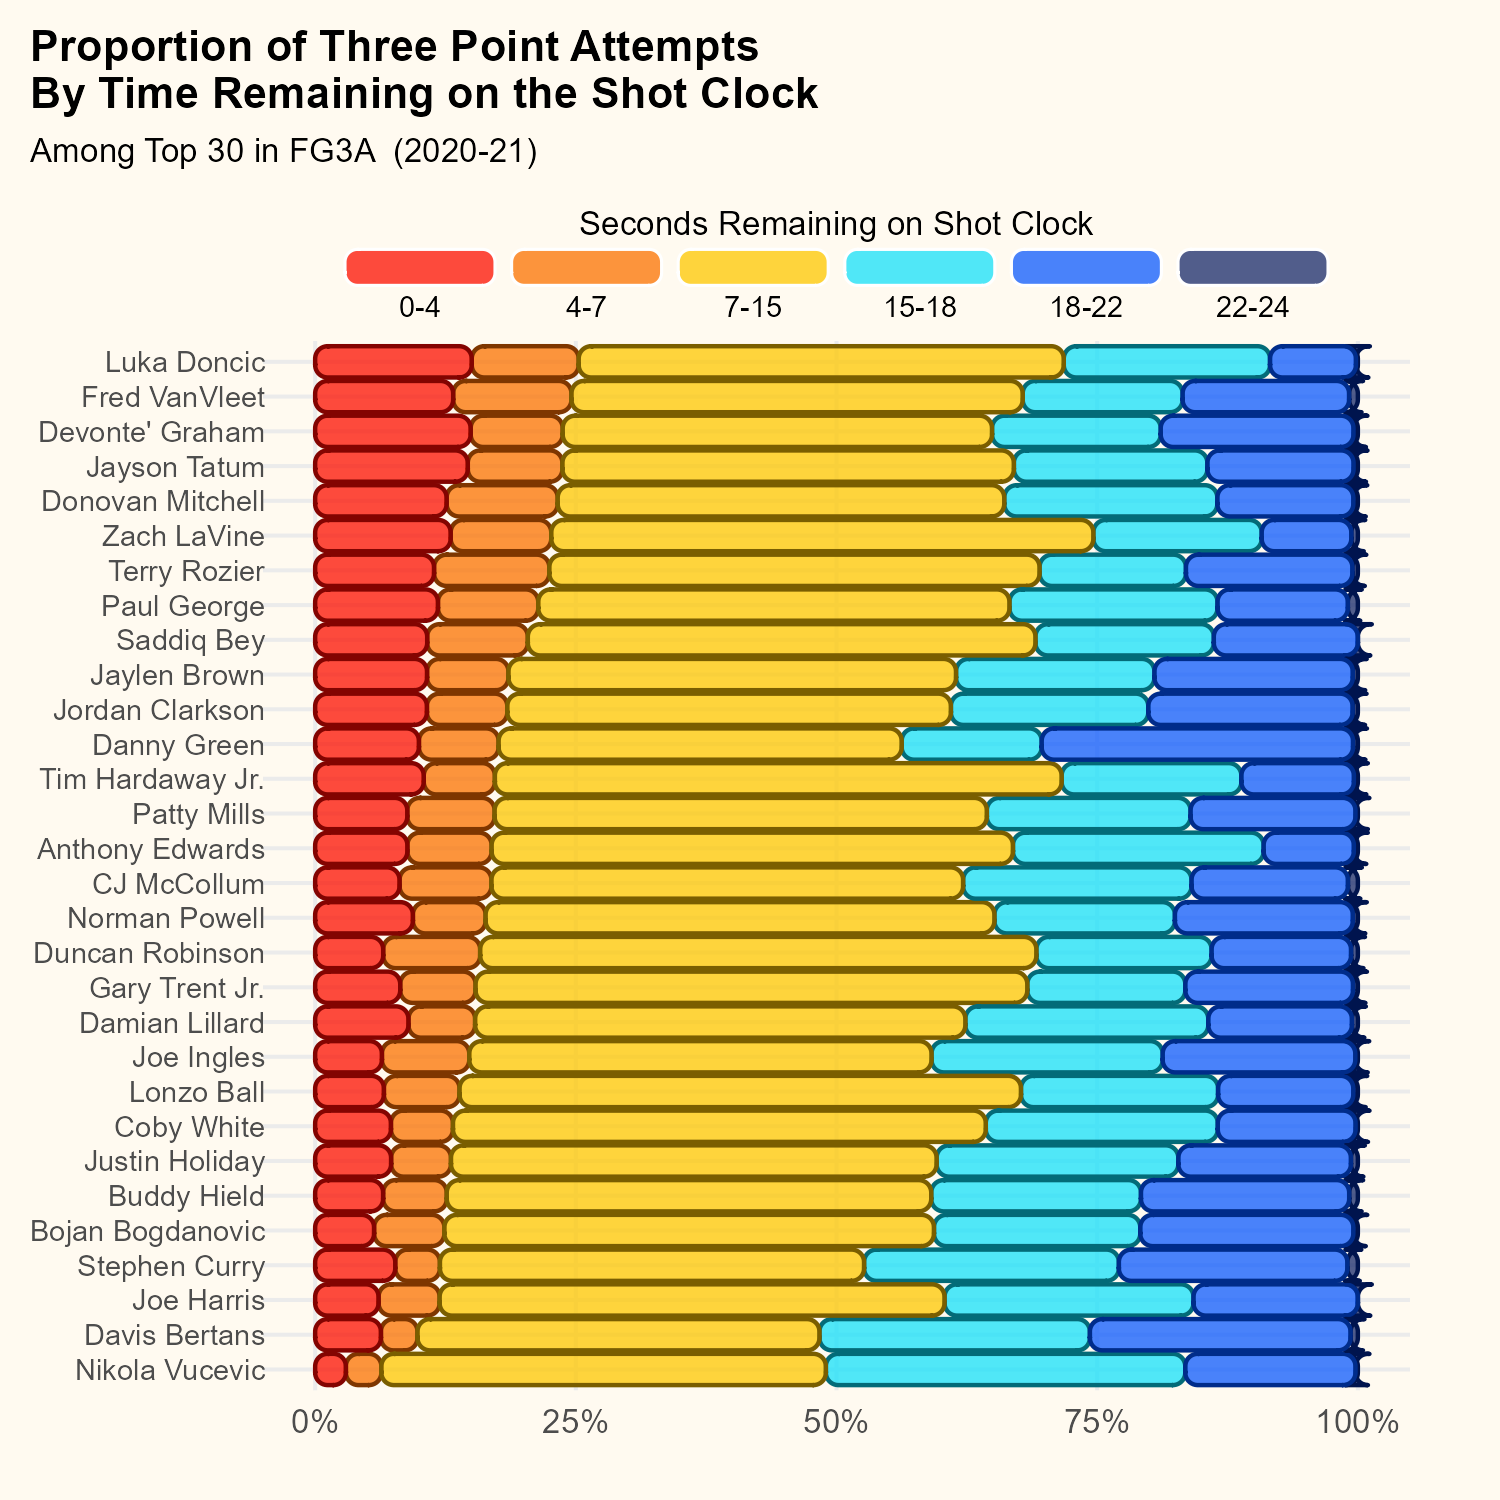
\includegraphics{./figures/hoopR_chicklet.png}
    
\end{figure}
\newpage
\section{\texttt{wehoop}}
\subsection{Data Sources}
As of \texttt{wehoop} version 1.1, the package exports \href{https://saiemgilani.github.io/wehoop/reference/index.html}{27 functions}. The prefix of exported functions generally indicates the data source of the package, so functions beginning with \texttt{espn\_} indicate that they are directly getting the data from the ESPN API, including those capable of use during live game-play for both women's college basketball and the WNBA.  
\subsection{WNBA full play-by-play seasons (2002-2021) ~ 1-2 minutes}
\texttt{\href{https://github.com/saiemgilani/The\_SportsDataverse\_Initiative/R/wehoop.R}{R/wehoop.R}}
\usemintedstyle{friendly}
\begin{minted}
[
baselinestretch=1.2,
bgcolor=offwhite,
fontsize=\footnotesize
]
{R}
tictoc::tic()
progressr::with_progress({
  wnba_pbp <- wehoop::load_wnba_pbp(2002:2021)
})
tictoc::toc()
## 12.01 sec elapsed
glue::glue("WNBA play-by-play data from {length(unique(wnba_pbp$game_id))} games.")
## WNBA play-by-play data from 4674 games.
# Rows: 1,782,985
# Columns: 42
#$ shooting_play             <lgl> FALSE, FALSE, TRUE, FALSE, TRUE, ~
#$ sequence_number           <chr> "1", "2", "3", "4", "5", "6", "7"~
#$ period_display_value      <chr> "1st Quarter", "1st Quarter", "1s~
#$ period_number             <int> 1, 1, 1, 1, 1, 1, 1, 1, 1, 1, 1, ~
#$ home_score                <int> 0, 0, 0, 0, 0, 0, 0, 0, 0, 0, 0, ~
#$ coordinate_x              <int> 0, 0, 35, 0, 40, 0, 0, 25, 0, 0, ~
#$ coordinate_y              <int> 0, 0, 11, 0, 5, 0, 0, 0, 0, 0, 0,~
#$ scoring_play              <lgl> FALSE, FALSE, FALSE, FALSE, FALSE~
#$ clock_display_value       <chr> "20:00", "20:00", "19:34", "19:31~
#$ team_id                   <chr> NA, "6", "6", "9", "9", "6", "6",~
#$ type_id                   <chr> "411", "615", "20558", "587", "20~
#$ type_text                 <chr> "Start Period", "Jumpball", "Jump~
#$ away_score                <int> 0, 0, 0, 0, 0, 0, 0, 2, 2, 2, 3, ~
#$ id                        <dbl> 22052500600000, 22052500600001, 2~
#$ text                      <chr> "Start of the 1st Half.", "Jumpba~
#$ score_value               <int> 0, 0, 0, 0, 0, 0, 0, 2, 0, 0, 1, ~
#$ participants_0_athlete_id <chr> NA, "18", "7", "21", "18", "6", "~
#$ participants_1_athlete_id <chr> NA, "6", NA, NA, NA, NA, "6", "20~
#$ participants_2_athlete_id <chr> NA, "9", NA, NA, NA, NA, NA, NA, ~
#$ type_abbreviation         <lgl> NA, NA, NA, NA, NA, NA, NA, NA, N~
#$ season                    <int> 2002, 2002, 2002, 2002, 2002, 200~
#$ season_type               <int> 2, 2, 2, 2, 2, 2, 2, 2, 2, 2, 2, ~
#$ away_team_id              <int> 9, 9, 9, 9, 9, 9, 9, 9, 9, 9, 9, ~
#$ away_team_name            <chr> "New York", "New York", "New York~
#$ away_team_mascot          <chr> "Liberty", "Liberty", "Liberty", ~
#$ away_team_abbrev          <chr> "NYL", "NYL", "NYL", "NYL", "NYL"~
#$ away_team_name_alt        <chr> "New York", "New York", "New York~
#$ home_team_id              <int> 6, 6, 6, 6, 6, 6, 6, 6, 6, 6, 6, ~
#$ home_team_name            <chr> "Los Angeles", "Los Angeles", "Lo~
#$ home_team_mascot          <chr> "Sparks", "Sparks", "Sparks", "Sp~
#$ home_team_abbrev          <chr> "LOS", "LOS", "LOS", "LOS", "LOS"~
#$ home_team_name_alt        <chr> "Los Angeles", "Los Angeles", "Lo~
#$ home_team_spread          <dbl> 2.5, 2.5, 2.5, 2.5, 2.5, 2.5, 2.5~
#$ game_spread               <dbl> 2.5, 2.5, 2.5, 2.5, 2.5, 2.5, 2.5~
#$ home_favorite             <lgl> TRUE, TRUE, TRUE, TRUE, TRUE, TRU~
#$ clock_minutes             <chr> "20", "20", "19", "19", "19", "19~
#$ clock_seconds             <chr> "00", "00", "34", "31", "21", "19~
#$ half                      <chr> "1", "1", "1", "1", "1", "1", "1"~
#$ lag_half                  <chr> NA, "1", "1", "1", "1", "1", "1",~
#$ lead_half                 <chr> "1", "1", "1", "1", "1", "1", "1"~
#$ game_play_number          <int> 1, 2, 3, 4, 5, 6, 7, 8, 9, 10, 11~
#$ game_id                   <int> 220525006, 220525006, 220525006, ~
\end{minted}

\subsection{WNBA full team box score seasons (2003-2021) ~ 5-30 seconds}
\usemintedstyle{friendly}
\begin{minted}
[
baselinestretch=1.2,
bgcolor=offwhite,
fontsize=\footnotesize
]
{R}
tictoc::tic()
progressr::with_progress({
  wnba_team_box <- wehoop::load_wnba_team_box(2003:2021)
})
tictoc::toc()
## 8.06 sec elapsed 
glue::glue("WNBA team boxscore data from {length(unique(wnba_team_box\$game_id))} games.")
## WNBA team boxscore data from 4312 games.
\end{minted}

\subsection{WNBA full player box score seasons (2002-2021) ~ 5-30 seconds}
\usemintedstyle{friendly}
\begin{minted}
[
baselinestretch=1.2,
bgcolor=offwhite,
fontsize=\footnotesize
]
{R}
tictoc::tic()
progressr::with_progress({
  wnba_player_box <- wehoop::load_wnba_player_box(2002:2021)
})
tictoc::toc()                    
## 6.68 sec elapsed
glue::glue("WNBA player boxscore data from {length(unique(wnba_player_box\$game_id))} games.")
## WNBA player boxscore data from 4677 games.
\end{minted}
\subsection{Women's college basketball full play-by-play seasons (2004-2021) ~ 45-90 seconds}
\usemintedstyle{friendly}
\begin{minted}
[
baselinestretch=1.2,
bgcolor=offwhite,
fontsize=\footnotesize
]
{R}
tictoc::tic()
progressr::with_progress({
  wbb_pbp <- wehoop::load_wbb_pbp(2004:2021)
})
tictoc::toc()                                                                                                           
## 44.51 sec elapsed
glue::glue("WBB play-by-play data from {length(unique(wbb_pbp$game_id))} games.")
## WBB play-by-play data from 26023 games.
dplyr::glimpse(wbb_pbp[1:53])
Rows: 8,650,487
Columns: 53
$ shooting_play                   <lgl> TRUE, FALSE, FALSE, TRUE, FALSE, TRUE, FALSE, TRUE, TRUE, FALSE, TRUE, FALSE, TRUE, FALSE, TRUE, ~
$ sequence_number                 <chr> "1", "2", "3", "4", "5", "6", "7", "8", "9", "10", "11", "12", "13", "14", "15", "16", "17", "18"~
$ period_display_value            <chr> "1st Half", "1st Half", "1st Half", "1st Half", "1st Half", "1st Half", "1st Half", "1st Half", "~
$ period_number                   <int> 1, 1, 1, 1, 1, 1, 1, 1, 1, 1, 1, 1, 1, 1, 1, 1, 1, 1, 1, 1, 1, 1, 1, 1, 1, 1, 1, 1, 1, 1, 1, 1, 1~
$ home_score                      <int> 0, 0, 0, 0, 0, 2, 2, 3, 5, 5, 5, 5, 5, 5, 6, 7, 9, 9, 9, 9, 9, 9, 9, 9, 9, 9, 10, 11, 11, 11, 11,~
$ scoring_play                    <lgl> FALSE, FALSE, FALSE, FALSE, FALSE, TRUE, FALSE, TRUE, TRUE, FALSE, FALSE, FALSE, TRUE, FALSE, TRU~
$ clock_display_value             <chr> "19:51", "19:51", "19:33", "19:18", "19:18", "19:13", "19:13", "19:13", "19:05", "18:57", "18:57"~
$ team_id                         <chr> "228", "150", "150", "228", "150", "150", "228", "150", "150", "150", "228", "228", "228", "228",~
$ type_id                         <chr> "20558", "587", "601", "20558", "587", "20558", "601", "97", "20424", "601", "97", "587", "97", "~
$ type_text                       <chr> "JumpShot", "Defensive Rebound", "Foul Turnover", "JumpShot", "Defensive Rebound", "JumpShot", "F~
$ away_score                      <int> 0, 0, 0, 0, 0, 0, 0, 0, 0, 0, 0, 0, 1, 1, 1, 1, 1, 1, 1, 1, 1, 1, 1, 1, 1, 1, 1, 1, 1, 1, 1, 1, 1~
$ id                              <dbl> 2405801500001, 2405801500002, 2405801500003, 2405801500004, 2405801500005, 2405801500006, 2405801~
$ text                            <chr> "Lakeia Stokes missed Two Point Jumper.", "Alana Beard Defensive Rebound.", "Foul on Mistie Bass"~
$ score_value                     <int> 0, 0, 0, 0, 0, 2, 0, 1, 2, 0, 0, 0, 1, 0, 1, 1, 2, 0, 0, 0, 0, 0, 0, 0, 0, 0, 1, 1, 0, 0, 0, 0, 2~
$ participants_0_athlete_id       <chr> "285", "436", "2475", "282", "2475", "438", "280", "438", "436", "438", "282", NA, "282", "280", ~
$ participants_1_athlete_id       <chr> NA, NA, NA, NA, NA, NA, NA, NA, NA, NA, NA, NA, NA, NA, NA, NA, NA, NA, NA, NA, NA, NA, NA, NA, N~
$ season                          <int> 2004, 2004, 2004, 2004, 2004, 2004, 2004, 2004, 2004, 2004, 2004, 2004, 2004, 2004, 2004, 2004, 2~
$ season_type                     <int> 2, 2, 2, 2, 2, 2, 2, 2, 2, 2, 2, 2, 2, 2, 2, 2, 2, 2, 2, 2, 2, 2, 2, 2, 2, 2, 2, 2, 2, 2, 2, 2, 2~
$ away_team_id                    <int> 228, 228, 228, 228, 228, 228, 228, 228, 228, 228, 228, 228, 228, 228, 228, 228, 228, 228, 228, 22~
$ away_team_name                  <chr> "Clemson", "Clemson", "Clemson", "Clemson", "Clemson", "Clemson", "Clemson", "Clemson", "Clemson"~
$ away_team_mascot                <chr> "Tigers", "Tigers", "Tigers", "Tigers", "Tigers", "Tigers", "Tigers", "Tigers", "Tigers", "Tigers~
$ away_team_abbrev                <chr> "CLEM", "CLEM", "CLEM", "CLEM", "CLEM", "CLEM", "CLEM", "CLEM", "CLEM", "CLEM", "CLEM", "CLEM", "~
$ away_team_name_alt              <chr> "Clemson", "Clemson", "Clemson", "Clemson", "Clemson", "Clemson", "Clemson", "Clemson", "Clemson"~
$ home_team_id                    <int> 150, 150, 150, 150, 150, 150, 150, 150, 150, 150, 150, 150, 150, 150, 150, 150, 150, 150, 150, 15~
$ home_team_name                  <chr> "Duke", "Duke", "Duke", "Duke", "Duke", "Duke", "Duke", "Duke", "Duke", "Duke", "Duke", "Duke", "~
$ home_team_mascot                <chr> "Blue Devils", "Blue Devils", "Blue Devils", "Blue Devils", "Blue Devils", "Blue Devils", "Blue D~
$ home_team_abbrev                <chr> "DUKE", "DUKE", "DUKE", "DUKE", "DUKE", "DUKE", "DUKE", "DUKE", "DUKE", "DUKE", "DUKE", "DUKE", "~
$ home_team_name_alt              <chr> "Duke", "Duke", "Duke", "Duke", "Duke", "Duke", "Duke", "Duke", "Duke", "Duke", "Duke", "Duke", "~
$ home_team_spread                <dbl> 2.5, 2.5, 2.5, 2.5, 2.5, 2.5, 2.5, 2.5, 2.5, 2.5, 2.5, 2.5, 2.5, 2.5, 2.5, 2.5, 2.5, 2.5, 2.5, 2.~
$ game_spread                     <dbl> 2.5, 2.5, 2.5, 2.5, 2.5, 2.5, 2.5, 2.5, 2.5, 2.5, 2.5, 2.5, 2.5, 2.5, 2.5, 2.5, 2.5, 2.5, 2.5, 2.~
$ home_favorite                   <lgl> TRUE, TRUE, TRUE, TRUE, TRUE, TRUE, TRUE, TRUE, TRUE, TRUE, TRUE, TRUE, TRUE, TRUE, TRUE, TRUE, T~
$ game_spread_available           <lgl> FALSE, FALSE, FALSE, FALSE, FALSE, FALSE, FALSE, FALSE, FALSE, FALSE, FALSE, FALSE, FALSE, FALSE,~
$ game_id                         <int> 240580150, 240580150, 240580150, 240580150, 240580150, 240580150, 240580150, 240580150, 240580150~
$ qtr                             <int> 1, 1, 1, 1, 1, 1, 1, 1, 1, 1, 1, 1, 1, 1, 1, 1, 1, 1, 1, 1, 1, 1, 1, 1, 1, 1, 1, 1, 1, 1, 1, 1, 1~
$ time                            <chr> "19:51", "19:51", "19:33", "19:18", "19:18", "19:13", "19:13", "19:13", "19:05", "18:57", "18:57"~
$ clock_minutes                   <chr> "19", "19", "19", "19", "19", "19", "19", "19", "19", "18", "18", "18", "18", "18", "18", "18", "~
$ clock_seconds                   <chr> "51", "51", "33", "18", "18", "13", "13", "13", "05", "57", "57", "57", "57", "47", "47", "47", "~
$ half                            <chr> "1", "1", "1", "1", "1", "1", "1", "1", "1", "1", "1", "1", "1", "1", "1", "1", "1", "1", "1", "1~
$ game_half                       <chr> "1", "1", "1", "1", "1", "1", "1", "1", "1", "1", "1", "1", "1", "1", "1", "1", "1", "1", "1", "1~
$ lag_qtr                         <dbl> NA, 1, 1, 1, 1, 1, 1, 1, 1, 1, 1, 1, 1, 1, 1, 1, 1, 1, 1, 1, 1, 1, 1, 1, 1, 1, 1, 1, 1, 1, 1, 1, ~
$ lead_qtr                        <dbl> 1, 1, 1, 1, 1, 1, 1, 1, 1, 1, 1, 1, 1, 1, 1, 1, 1, 1, 1, 1, 1, 1, 1, 1, 1, 1, 1, 1, 1, 1, 1, 1, 1~
$ lag_game_half                   <chr> NA, "1", "1", "1", "1", "1", "1", "1", "1", "1", "1", "1", "1", "1", "1", "1", "1", "1", "1", "1"~
$ lead_game_half                  <chr> "1", "1", "1", "1", "1", "1", "1", "1", "1", "1", "1", "1", "1", "1", "1", "1", "1", "1", "1", "1~
$ start_quarter_seconds_remaining <int> 1191, 1191, 1173, 1158, 1158, 1153, 1153, 1153, 1145, 1137, 1137, 1137, 1137, 1127, 1127, 1127, 1~
$ start_half_seconds_remaining    <int> 1791, 1791, 1773, 1758, 1758, 1753, 1753, 1753, 1745, 1737, 1737, 1737, 1737, 1727, 1727, 1727, 1~
$ start_game_seconds_remaining    <int> 2991, 2991, 2973, 2958, 2958, 2953, 2953, 2953, 2945, 2937, 2937, 2937, 2937, 2927, 2927, 2927, 2~
$ game_play_number                <int> 1, 2, 3, 4, 5, 6, 7, 8, 9, 10, 11, 12, 13, 14, 15, 16, 17, 18, 19, 20, 21, 22, 23, 24, 25, 26, 27~
$ end_quarter_seconds_remaining   <dbl> 600, 1191, 1191, 1173, 1158, 1158, 1153, 1153, 1153, 1145, 1137, 1137, 1137, 1137, 1127, 1127, 11~
$ end_half_seconds_remaining      <dbl> 1200, 1791, 1791, 1773, 1758, 1758, 1753, 1753, 1753, 1745, 1737, 1737, 1737, 1737, 1727, 1727, 1~
$ end_game_seconds_remaining      <dbl> 2400, 2991, 2991, 2973, 2958, 2958, 2953, 2953, 2953, 2945, 2937, 2937, 2937, 2937, 2927, 2927, 2~
$ period                          <int> 1, 1, 1, 1, 1, 1, 1, 1, 1, 1, 1, 1, 1, 1, 1, 1, 1, 1, 1, 1, 1, 1, 1, 1, 1, 1, 1, 1, 1, 1, 1, 1, 1~
$ coordinate_x                    <int> NA, NA, NA, NA, NA, NA, NA, NA, NA, NA, NA, NA, NA, NA, NA, NA, NA, NA, NA, NA, NA, NA, NA, NA, N~
$ coordinate_y                    <int> NA, NA, NA, NA, NA, NA, NA, NA, NA, NA, NA, NA, NA, NA, NA, NA, NA, NA, NA, NA, NA, NA, NA, NA, N~

\end{minted}

\subsection{Women's college basketball full team box score seasons (2006-2021) ~ 5-30 seconds}
\usemintedstyle{friendly}
\begin{minted}
[
baselinestretch=1.2,
bgcolor=offwhite,
fontsize=\footnotesize
]
{R}
tictoc::tic()
progressr::with_progress({
  wbb_team_box <- wehoop::load_wbb_team_box(2006:2021)
})
tictoc::toc()
## 7.12 sec elapsed
glue::glue("WBB team boxscore data from {length(unique(wbb_team_box$game_id))} games.")
## WBB team boxscore data from 20762 games.
\end{minted}


\subsection{Women's college basketball full player box score seasons (2006-2021) ~ 5-30 seconds}

\usemintedstyle{friendly}
\begin{minted}
[
baselinestretch=1.2,
bgcolor=offwhite,
fontsize=\footnotesize
]
{R}
tictoc::tic()
progressr::with_progress({
  wbb_player_box <- wehoop::load_wbb_player_box(2006:2021)
})
tictoc::toc()
glue::glue("WBB player boxscore data from {length(unique(wbb_player_box$game_id))} games.")
\end{minted}

\section{What next?}
The first phase of the initiative is to broaden the number of sports the packages covered by the packages through existing data sources, to improve the quality of the existing packages, and to recruit existing open-source sports data packages and their developers to the organization.

The end goal of the initiative would allow the interested to get started in sports analytics with a command as simple as: 
\usemintedstyle{friendly}
\begin{minted}
[
baselinestretch=1.2,
bgcolor=offwhite,
fontsize=\footnotesize
]
{R}
# Python (already possible, go try it)
pip install sportsdataverse
# R (Work in progress)
install.packages(sportsdataverse)
# Node.js (already possible, go try it)
yarn add sportsdataverse
\end{minted}

For a thorough covering of the documentation for each of the packages and their functionalities, please refer to Table \ref{tbl:sdvpy} for the Python packages, Table \ref{tbl:sdvr} for the R packages, and Table \ref{tbl:sdvjs} for the Node.js modules. 
\newpage
\section{Package Documentation Reference}
These are the packages that have agreed to join us the SportsDataverse:
\begin{table}[!htbp]
\centering
\renewcommand{\arraystretch}{1.3}
\begin{tabular}{>{\raggedright}m{1.0in} >{\raggedright}m{2.2in} >{\centering}m{0.8in} >{\raggedright\arraybackslash}m{2.0in}}
\toprule
\multicolumn{4}{c}{\textbf{Python Packages in the SportsDataverse}} \\
\textbf{Package} & \textbf{Sports Leagues} & \textbf{Repository} & \textbf{Author(s)} \\ 
 \midrule
    sportsdataverse & College Football, NFL, NBA, WNBA, NHL, Men's and Women's College Basketball, most collegiate sports & \href{https://github.com/saiemgilani/sportsdataverse-py/}{GitHub} - \href{https://py.sportsdataverse.org/}{Docs} & Saiem Gilani\\
\bottomrule
\end{tabular}
\vspace{5pt}
\caption{Python packages contributed to the SportsDataverse}
\label{tbl:sdvpy}
\vspace{-7mm}
\end{table}
\begin{table}[!htbp]
\centering
\renewcommand{\arraystretch}{1.3}
\begin{tabular}{>{\raggedright}m{1.0in} >{\raggedright}m{2.2in} >{\centering}m{0.8in} >{\raggedright\arraybackslash}m{2.0in}}
\toprule
\multicolumn{4}{c}{\textbf{R Packages in the SportsDataverse}} \\
\textbf{Package} & \textbf{Sports Leagues} & \textbf{Repository} & \textbf{Author(s)} \\ 
 \midrule
    cfbfastR & College Football & \href{https://github.com/saiemgilani/cfbfastR/}{GitHub} - \href{https://saiemgilani.github.io/cfbfastR/}{Docs} & Saiem Gilani, Akshay Easwaran, Jared Lee, Eric Hess \\
    gamezoneR  & Men's and Women's College Basketball & \href{https://github.com/jacklich10/gamezoneR/}{GitHub} - \href{https://jacklich10.github.io/gamezoneR/}{Docs} & Jack Lichtenstein \\
    hoopR & NBA and Men's College Basketball & \href{https://github.com/saiemgilani/hoopR/}{GitHub} - \href{https://hoopR.sportsdataverse.org}{Docs} & Saiem Gilani \\
    puntr & NFL and College Football & \href{https://github.com/Puntalytics/puntr}{GitHub} - \href{https://puntalytics.github.io/puntr/}{Docs} & Dennis Brookner and Raphael LadenGuindon \\
    recruitR & Men's College Sports Recruiting & \href{https://github.com/saiemgilani/recruitR/}{GitHub} - \href{https://saiemgilani.github.io/recruitR/}{Docs} & Saiem Gilani \\
    wehoop & WNBA and Women's College Basketball & \href{https://github.com/saiemgilani/wehoop}{GitHub} - \href{https://wehoop.sportsdataverse.org}{Docs} & Saiem Gilani and Geoff Hutchinson \\
    worldfootballR & EPL, La Liga, Bundesliga, Serie A, Ligue 1, RFPL & \href{https://github.com/JaseZiv/worldfootballR}{GitHub} - \href{https://jaseziv.github.io/worldfootballR}{Docs} & Jason Zivkovic \\
    baseballr & MLB, MiLB, NCAA Baseball & \href{https://github.com/BillPetti/baseballr/}{GitHub} - \href{https://BillPetti.github.io/baseballr}{Docs} & Bill Petti \\
    hockeyR & NHL & \href{https://github.com/danmorse314/hockeyR/}{GitHub} - \href{https://hockeyr.netlify.app/}{Docs} & Dan Morse \\
    fastRhockey & NHL & \href{https://github.com/BenHowell71/fastRhockey/}{GitHub} - \href{https://BenHowell71.github.io/fastRhockey}{Docs} & Ben Howell \\
    powerplay & NHL & \href{https://github.com/saiemgilani/powerplay}{GitHub} - \href{https://saiemgilani.github.io/powerplay}{Docs} & Saiem Gilani \\
\bottomrule 
\end{tabular}
\vspace{5pt}
\caption{R Packages contributed to the SportsDataverse}
\label{tbl:sdvr}
\vspace{-7mm}
\end{table}
\begin{table}[!htbp]
\centering
\renewcommand{\arraystretch}{1.3}
\begin{tabular}{>{\raggedright}m{1.0in} >{\raggedright}m{2.2in} >{\centering}m{0.8in} >{\raggedright\arraybackslash}m{2.0in}}
\toprule
\multicolumn{4}{c}{\textbf{Node.js Packages in the SportsDataverse}} \\
\textbf{Package} & \textbf{Sports Leagues} & \textbf{Repository} & \textbf{Author(s)} \\ 
 \midrule
    sportsdataverse & College Football, NFL, NBA, WNBA, NHL, Men's and Women's College Basketball, most collegiate sports & \href{https://github.com/saiemgilani/sportsdataverse}{GitHub} - \href{https://saiemgilani.github.io/sportsdataverse}{Docs} & Saiem Gilani\\
    nfl-nerd & NFL & \href{https://github.com/nntrn/nfl-nerd}{GitHub} & Annie Tran \\
\end{tabular}
\vspace{5pt}
\caption{Node.js modules contributed to the SportsDataverse}
\label{tbl:sdvjs}
\vspace{-7mm}
\end{table}
\newpage
% \subsection{Package Logos}\begin{figure}[htbp]
%     \centering
%     \caption{cfbfastR, hoopR, wehoop in \textit{R, Python}}
%     \centering
%     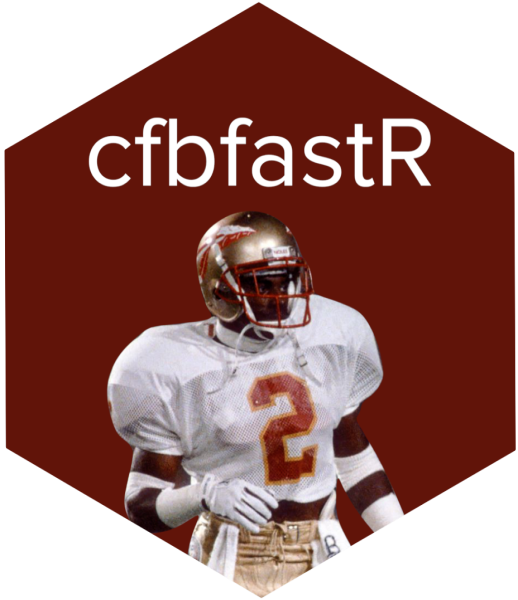
\includegraphics[width=0.1\textwidth]{./figures/cfbfastR.png}
%     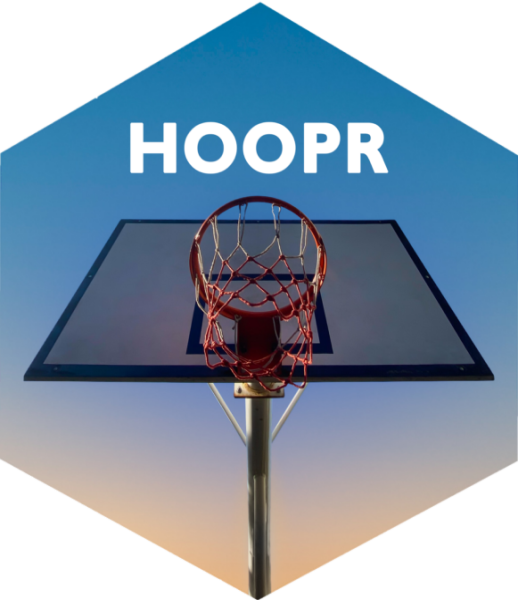
\includegraphics[width=0.1\textwidth]{./figures/hoopR.png}
%     
\includegraphics[width=0.1\textwidth]{./figures/wehoop.png}
%     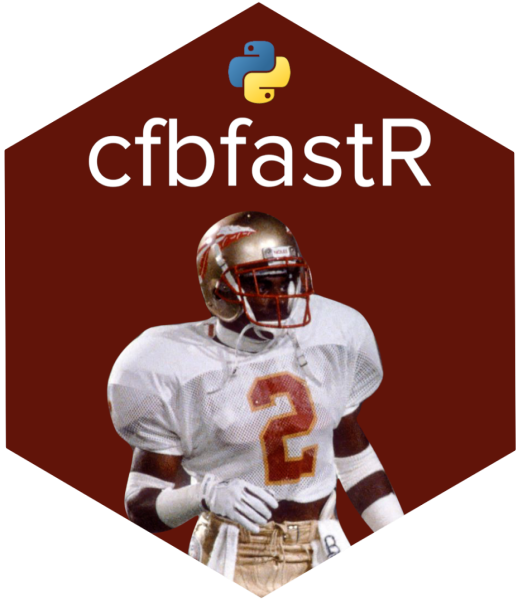
\includegraphics[width=0.1\textwidth]{./figures/cfbfastR-py.png}
%     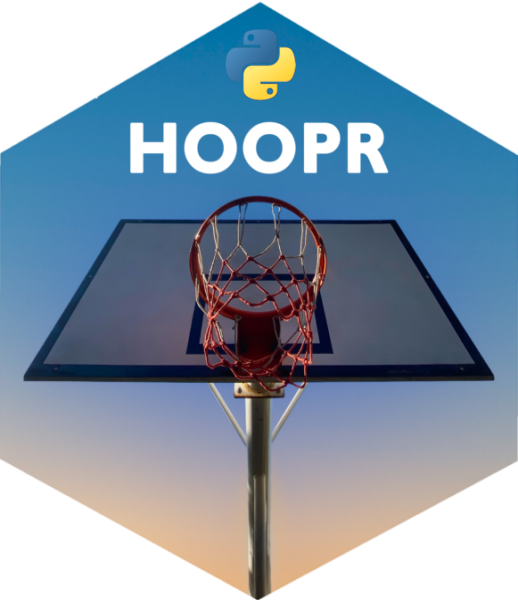
\includegraphics[width=0.1\textwidth]{./figures/hoopR-py.png}
%     
\includegraphics[width=0.1\textwidth]{./figures/wehoop-py.png}
%     \label{fig:sdvR}
% \end{figure} 
% \newpage
\section{References}
\printbibliography[title={\hspace{5pt}\vspace{-10pt}}]

\end{document}
